\section{Contraposée du théorème de Thalès}
    \subsection{Énoncé}
        \begin{theoreme}[\admis]
            Si dans une configuration géométrique :
            \begin{itemize}
                \item Deux droites $(d)$ et $(d')$ sont sécantes en un point $A$.
                \item $B$ et $M$ sont deux points de la droites $(d)$, distincts de A.
                \item $C$ et $N$ sont deux points de la droite $(d')$, distincts de $A$.
                \item $\dfrac{AM}{AB} \neq \dfrac{AN}{AC}$.       
            \end{itemize}
            \medskip
            alors les droites $(BC)$ et $(MN)$ ne sont pas parallèles.
        \end{theoreme}

        \begin{remarque}
            D'une façon générale, la contraposée d'un théorème permet d'affirmer que les conditions
            de ce théorème sont fausses dès que l'unes des condittions nécessaires à l'application de ce théorème l'est.

            En effet, ici, si les droites étaient parallèles alors les rapports $\dfrac{AB}{AM}$ , $\dfrac{AC}{AN}$ et $\dfrac{BC}{MN}$ seraient égaux
            or $\dfrac{AM}{AB} \neq \dfrac{AN}{AC}$ fait parties des hypothèses du théorème donc les trois rapports ne peuvent 
            être égaux ce qui signifie que les droites $(BC)$ et $(MN)$ ne peuvent être parallèles.
        \end{remarque}
    
    \subsection{Exemple de rédaction}

        \begin{methode*1}[Justifier que deux droites ne sont pas parallèles]
            \begin{multicols}2
                \begin{itemize}
                    \item Déterminer les droites sécantes.                    
                    \item Identifier les deux triangles de la configurations.
                    \columnbreak
                    \item Calculer les rapports de longueurs correspondantes non portées par les droites candidates.
                    \item Invoquer la contraposée du théorème de Thalès ou le théorème lui-même.
                \end{itemize}
            \end{multicols}

            \exercice

            \begin{minipage}{8cm}
                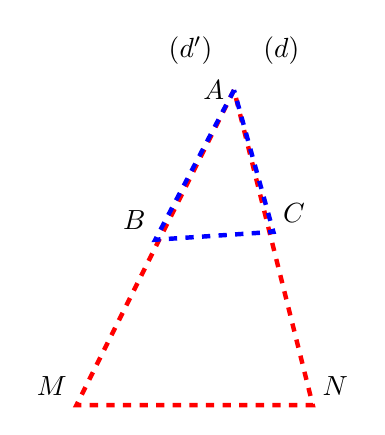
\begin{tikzpicture}[scale = 0.5]
                    % \draw[help lines, color=black!30, dashed] (0,0) grid (12,14);        
                    \coordinate[label=left:$A$] (A) at (7,13);
                    \coordinate[label=left:$(d')$] (d') at (6.7,14);
                    \coordinate[label=right:$(d)$] (d) at (7.5,14);
                    \coordinate[label=above right:$N$] (N) at (9,5);
                    \coordinate[label=above left:$M$] (M) at (3,5);
                    \coordinate[label=above left:$B$] (B) at (5,9.2);
                    \coordinate (M1) at (4,5);
                    \coordinate[label=above right:$C$] (C) at (8,9.4);
                    \coordinate (N1) at (10,5);
        
                    \tkzDrawLine(A,M);
                    \tkzDrawLine(A,N);
                    \tkzDrawLine(M,N);
                    \tkzDrawLine(B,C);
                    \tkzDrawLine(M1,N1);     
                    \draw[dashed, color=red, ultra thick] (A)--(M)--(N)--(A);
                    \draw[dashed, color=blue, ultra thick] (A)--(B)--(C)--(A);
                \end{tikzpicture}
            \end{minipage}
            \begin{minipage}{8cm}
                \begin{itemize}
                    \item Les droites $(d)$ et $(d')$ se coupent en $A$.
                    \item $AB=\Lg{11.9}$ ; $AM=\Lg{35}$ ; $AC=\Lg{18.2}$ ; $AN=\Lg{52}$
                \end{itemize}

                \vspace*{1cm}
                Démontrer que les droites $(MN)$ et $(BC)$ ne sont pas parallèles.
            \end{minipage}
            
            \correction
            Dans la configuration ci-dessus : 
            \begin{itemize}
                \item les droites $(MB)$ et $(CN)$ sont sécantes en $A$.                
                \item les deux triangles de la configurations sont \textcolor{red}{$AMN$} et \textcolor{blue}{$ABC$}.
            \end{itemize}
            \begin{spacing}2
                D'une part $\dfrac{\textcolor{blue}{AB}}{\textcolor{red}{AM}} = \dfrac{\textcolor{blue}{11,9}}{\textcolor{blue}{35}}=0,34$

                D'autre part $\dfrac{\textcolor{blue}{AC}}{\textcolor{red}{AN}} = \dfrac{\textcolor{blue}{18,2}}{\textcolor{blue}{52}}=0,35$
            \end{spacing}

            \begin{remarque}
                Les deux rédactions suivantes sont valables.
            \end{remarque}
            
            \hspace*{0.5cm}

            \begin{minipage}{8cm}
                \textbf{or}, si le droites $(MN)$ et $(BC)$ étaient parallèles, d'après le théorème de Thalès, il y aurait égalité des deux rapports
                précédents. Comme ce n'est pas le cas, c'est que \psshadowbox{les droites $(MN)$ et $(BC)$ ne sont pas parallèles}.
    
            \end{minipage}
            \hspace*{0.5cm}
            \vrule
            \hspace*{0.5cm}
            \begin{minipage}{8cm}
                Les rapports précédents étant différents, d'après la contraposée du théorème de Thalès, on peut conclure que \psshadowbox{les droites $(MN)$ et $(BC)$ ne sont pas parallèles}.
            \end{minipage}
        \end{methode*1}


% \subsection{Sous-section 1.1}
% \begin{definition}[Titre optionnel]
%     Dans le cours, on utilise assez souvent des cadres du type
%     définition (comme ici par exemple).    
% \end{definition}
% \begin{remarque}
%     Ceci est une remarque utilisant une commande du paquet profcollege.
    
%     \begin{center}
%       Truc centré
%     \end{center}


% \end{remarque}
% \begin{propriete}[Titre optionnel]
%   Dans le cours, on utilise assez souvent des cadres du type
%   définition, comme ici par exemple pour une propriete.
% \end{propriete}
% \begin{remarques}
%   \begin{itemize}
%     \item remarque.
%     \item remarque.
%   \end{itemize}
% \end{remarques}

% \subsection{Sous-section 1.2}
% \begin{theoreme}[Titre optionnel]
%   Dans le cours, on utilise assez souvent des cadres du type
%   définition, comme ici par exemple pour un théorème.
% \end{theoreme}
% \begin{notation}
%   notation
% \end{notation}
% \begin{notations}
%   \begin{itemize}
%     \item notation.
%     \item notation.
%   \end{itemize}
% \end{notations}
% \begin{preuve}
%   Ceci est une preuve\par Deuxième ligne de la preuve
% \end{preuve}
% \begin{exemple}
%   Texte de l’exemple
%   \correction
  
% \end{exemple}

% \begin{exemple*1}
%   \phantom{rrr}
%   Texte

%   \correction
%   \phantom{rrr}
%   Texte  
  
% \end{exemple*1}

% \begin{exemple}[0.6]
%   Texte de l’exemple très long sur une ligne, très très très long.
%   On peut modifier la répartition horizontale  à l'aide d'un argument optionnel valant par défaut 0,4, valant ici 0,6.
%   \correction
%   Texte de la correction en vis à vis
% \end{exemple}
% \section{Section 2}
% \subsection{Sous-section 2.1}
% Quatre affichages prévus pour les méthodes.

% \begin{methode}[Titre de la méthode]
%     \Papiers[Largeur=10,Hauteur=5,Couleur=Olive]
    
%     Texte introductif
%     \exercice
%     Texte de l’exercice
%     \correction
%     Texte de la correction sur un minimum de trois lignes pour faire la
%     différence entre vis-à-vis et double colonne. C’est l’endroit de la
%     coupure qui va différer.
% \end{methode}

% \begin{methode*1}[Titre de la méthode*1]
%     Texte introductif
%     \exercice
%     Texte de l’exercice
%     \correction
%     Texte de la correction sur un minimum de trois lignes pour faire la
%     différence entre vis-à-vis et double colonne. C’est l’endroit de la
%     coupure qui va différer.
% \end{methode*1}

% \subsection{Sous-section 2.2}
% \begin{methode*2}[Titre de la méthode*2]
%     Texte introductif
%     \exercice
%     Texte de l’exercice
%     \correction
%     Texte de la correction sur un minimum de trois lignes pour faire la
%     différence entre vis-à-vis et double colonne. C’est l’endroit de la
%     coupure qui va différer.
% \end{methode*2}

% \begin{methode*2*2}[Dernière méthode  \MethodeRefExercice{exoN1-exemple1} \MethodeRefExercice{exoN1-exemple2}]
%     \exercice
%     \label{methodeN1-exemple}
%     Texte du premier exercice
%     \correction
%     Correction du premier exercice
%     \exercice
%     Texte du deuxième exercice
%     \correction
%     Texte de la correction du deuxième exercice sur un minimum de trois
%     lignes pour faire la différence entre vis-à-vis et double
%     colonne. C’est l’endroit de la coupure qui va différer.
% \end{methode*2*2}